\section{Introducción}
Los asistentes inteligentes están buscando su hueco en todo hogar, y esto es un hecho.
Estos asistentes nos hacen la vida más sencilla, ayudando a actualizar y controlar toda la domótica de nuestras casas con acciones que hace unos años solo podíamos imaginarlas en películas de ciencia ficción.

El concepto de asistentes de voz, que tan de moda está ahora entre la población joven, junto con la gente de edad avanzada que necesita interacción en sus vidas puede ser una combinación perfecta para ayudarles a no perder el contacto con la sociedad.

La creación de un asistente que pueda resolver sus dudas, con el que puedan hablar, al que puedan preguntar a qué hora es la partida de cartas en el bar, o al que puedan pedir auxilio en caso de una caída, puede ser de gran utilidad para mejorar su día a día, al igual que servir de alivio para el resto de familiares que no pueden estar cerca de sus seres queridos, sabiendo que van a poder ser informados rápidamente de un posible accidente.

Pero el auge de los dispositivos asistentes pone en vilo la gestión de la privacidad e intimidad que hay dentro de nuestras casas,n y todo esto es debido a que pueden recolectar información a través de escuchar las conversaciones de nuestro día a día, siendo información que no sabemos a dónde va a parar, qué se va a hacer con ella.

Esta información es de un caracter sensible, ya que puede contener desde nuestros simples gustos, incluyendo nuestras necesidades, hasta nuestras tendencias políticas, siendo datos que pueden estar siendo utilizados por terceros, o incluso siendo vendidos ante nuestro desconocimiento.

La falta de soluciones en el mercado que cumplan todos estos puntos suponen una motivación para la creación de un asistente que no esté conectado constantemente a internet, ya que las personas de edad avanzada seguramente no tengan contratado el servicio, y que tampoco almacene datos de carácter sensible de los usuarios, sino que simplemente interaccione con cada persona, y la ayude en su día a día, tanto ofreciendo actividades de la misma localidad, como respondiendo cualquier pregunta que pase por la cabeza de quien lo posea, al igual que buscando ayuda en caso de que una persona requiera auxilio.

Antes de adentrar en la elección de un asistente inteligente, se expondrá qué es, y cuál es su funcionamiento, para entender mejor los motivos por los cuales se acaba eligiendo uno en vez de otro.

\subsubsection{Qué es un asistente inteligente}

Un asistente inteligente es simplemente una máquina programada de manera que su comportamiento se asemeje al de una persona a la que se solicita asistencia, como su propio nombre indica, pudiendo mantener una conversación que siga los protocolos de comunicación humana.

\begin{figure}[h!]
    \centering
    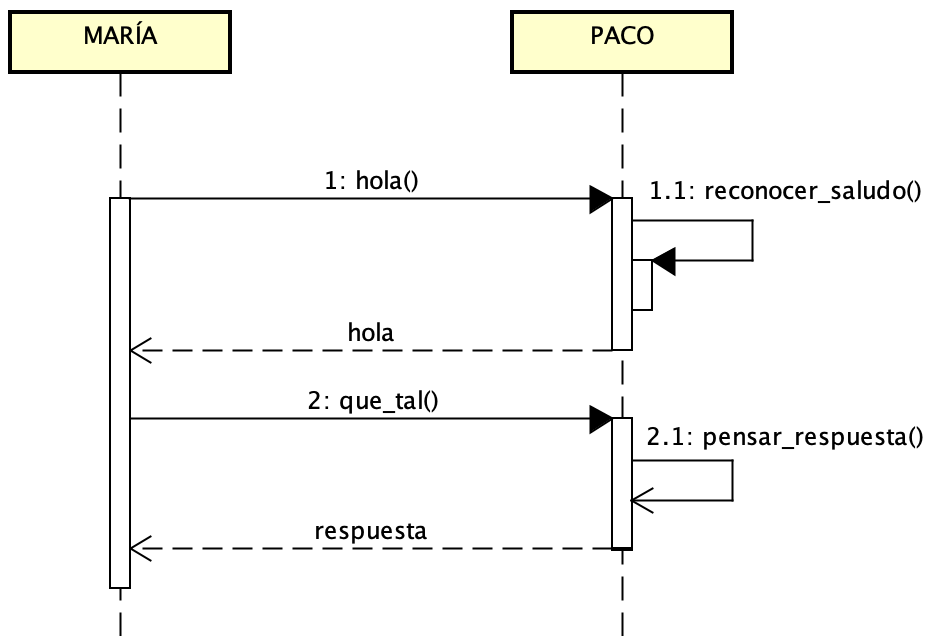
\includegraphics[width=10cm]{./img/sequence/human.png}
    \caption{Secuencia de comunicación humana}
    \label{fig:humanseq}
\end{figure}

Como se puede ver en la figura \ref{fig:humanseq}, un protocolo de comunicación entre dos personas se basaría en un saludo para entablar conversación, para posteriormente realizar una pregunta.

En el caso de los asistentes, el proceso de conversación se basa en lo mismo: un usuario saluda al asistente mediante el uso de una palabra o conjunto de palabras, al que se llamará \textbf{hotword}, que cuando sea reconocido por el asistente inteligente, devolverá el saludo.
Es entonces cuando el usuario debe realizar la pregunta o solicitar la información que requiera.
Una vez hecha la pregunta, el dispositivo se pondrá a pensar la posible respuesta, entrando en el proceso al que se llamará \textbf{reconocimiento de los hechos}. Una vez identificados los hechos, devolverá la respuesta que más se acerque a lo deseado, gracias a un entrenamiento previo.

\subsubsection{Cómo piensa el asistente}

El proceso de pensamiento analizado entre los principales asistentes, que se expondrá en este capítulo tiene una estructura similiar independientemente del tipo de asistente que se trate, asemejándose a la figura \ref{fig:humasseq}.

\begin{figure}[h!]
    \centering
    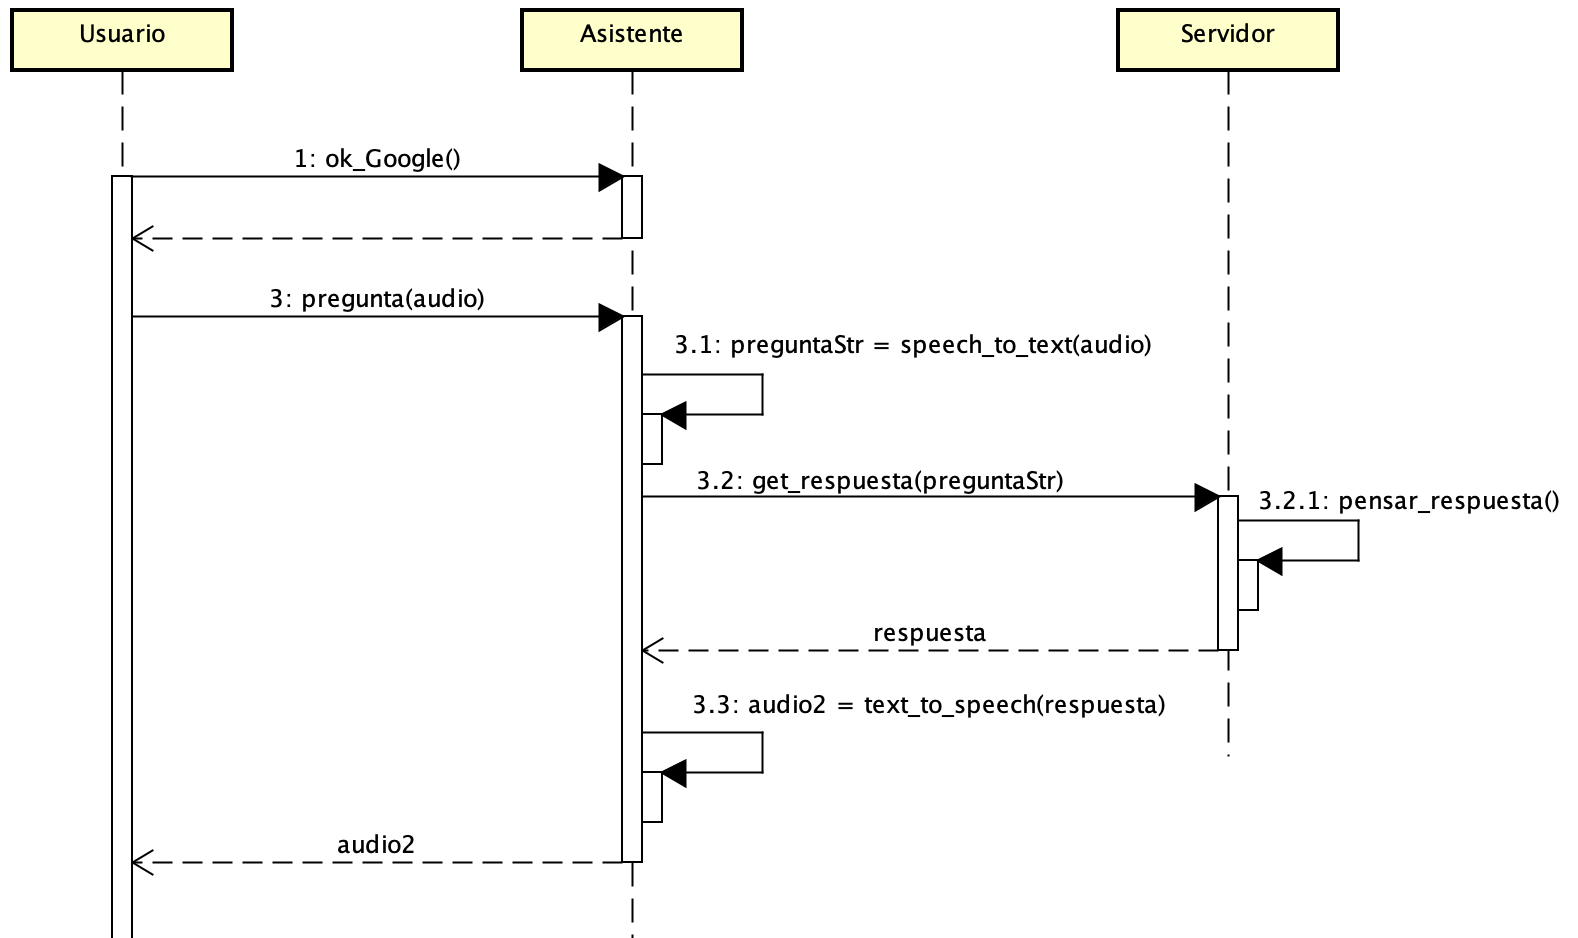
\includegraphics[width=14cm]{./img/sequence/humasseq.png}
    \caption{Secuencia de comunicación humano-asistente}
    \label{fig:humasseq}
\end{figure}

Lo que diferencia a un asistente de otro, es la manera en la cual piensa la respuesta, dando mayor validez a un asistente que dé una respuesta más aproximada a lo solicitado.
Para esto, la mayoría de asistentes tienen el procesamiento de la respuesta en la nube debido a la gran cantidad de información que tienen almacenada para contrastar los hechos capturados, al igual que también tienen en la nube el proceso de speech-to-text o el de text-to-speech.


\section{Requisitos mínimos}
Una vez que ya se ha expuesto cual es el funcionamiento base de un asistente virtual inteligente, interesa saber cual es que más se adecúa a las necesidades establecidas para este proyecto, de manera que se le exijirá que cumpla el máximo de los siguientes puntos expuestos.

\subsubsection{Despliegue en dispositivos}

El asistente seleccionado debe poder ser desplegado de manera gratuíta en un dispositivo formado por una placa RasbperryPi, o similar.

Para ello, se requiere que el asistente disponga de una librería o de un modo de uso que se pueda implementar en un dispositivo pequeño y portátil, facilitando el cambio de una ubicación física por otra de los distintos posibles lugares que existen dentro de un hogar, manteniendo una instalación lo más simple y limpia posible, en la que solo sea requerida la localización de un enchufe a la toma de la luz.

\subsubsection{Tratamiento de la información}

El asistente debe seguir la ley orgánica de protección de datos, y no debe tener acceso a escuchar conversaciones ajenas violando la intimidad de los usuarios.

Cualquier vacío legal o conjunto de cláusulas de extensa longitud no podrá será aceptado, para poder asegurar la protección de los datos de los usuarios.

En caso de almacenar algún tipo de dato, debe poder ser público para el usuario en cuestión, o haber sido aceptado expresamente por el usuario a favor de un control de su seguridad.

\subsubsection{Conexión a Internet}

La orientación de un dispositivo asistente inteligente como este a personas de una edad avanzada debe tener en cuenta que es posible que la mayoría de sus usuarios potenciales no tengan una conexión a internet en sus respectivos hogares.

Esto provoca que la conexión del dispositivo a la red tiene que ser lo mínima posible, favoreciendo los asistentes en los cuales el proceso de pensamiento sea ejecutado dentro del propio dispositivo, evitando tener que hacer el cálculo e identificación en servidores de alojados en la nube.

Es decir, el dispositivo debe ser capaz de funcionar en el lugar más remoto posible y sin ninguna conexión a internet, simplemente tras ser conectado a una red eléctrica.

\subsubsection{Adicción de nuevas tareas}

El software del asistente inteligente debe tener la capacidad de añadir nuevas tareas fácilmente, de modo que se puedan añadir nuevas funciones tanto propias, como desarrolladas por la comunidad de Internet.

\section{Mercado}
En los siguientes apartados se mostrarán las diferentes opciones que ofrece ya el mercado para el uso de asistentes inteligentes, con el fin de comprobar la existencia de alguno que ya tenga establecidos los requisitos base ya descritos, o que permita la opción de poder establecerlos.

    \subsection{Google Assistant}
    El asistente inteligente de Google es el que está en el año 2020 a la cabeza de los asistentes virtuales********ENLACE********, y esto es debido a que viene instalado en todos los dispositivos Android, ocupando estos dispositivos la mayor parte del mercado de la telefonía móvil. Esta posición privilegiada le da un mayor entrenamiento, elevando el acierto y usabilidad de este.

La creación de Google tiene una gran aceptación con los diferentes aparáticos de la domótica del hogar, facilitando la implementación y realización de tareas:

- Una tarea es un conjunto de acciones que se llevan a cabo tras accionarse un evento que hace de interruptor, pudiendo ser el evento tanto un comando de voz, la pulsación de un interruptor o la activación de un sensor, entre otras opciones.

De esta manera, Google permite el control de la domótica del hogar, o la realización de diferentes acciones en nuestro día a día, pero requiere ser configurado por cada usuario, evitando por tanto la posibilidad de un despliegue común.

\subsubsection{Cómo funciona}

El proceso de pensamiento que hace el asistente de Google está basado en la nube, pero no solo eso sino que Google hace en sus servidores también el proceso de Speech-to-Text.

De este modo, Google almacena todos los audios que se le mandan a través de su asistente, estudiándolos uno a uno y asegurando o corrigiendo sobre la respuesta que envió el asistente.

Este proceso de corregir o confirmar es el método que tiene Google de entrenamiento, de manera que en la próxima consulta sobre el mismo tema, el asistente pueda responder con mayor exactitud.

Queda claro que sobre la teoría es un buen plan de entrenamiento, y en un mundo ideal esto sería perfecto, pero esos audios también pueden contener parte de información privada, o pueden servir para espiar conversaciones privadas que un usuario puede no querer que estén almacenadas, ni que sean escuchadas por otra persona, aunque sea un propio trabajador.

https://elpais.com/tecnologia/2019/07/18/actualidad/1563466196_049167.html

En cuanto a la posibilidad de ser desplegado en otro dispositivo que no sea un smartphone o una tablet, Google nos lo pone fácil, ya que otorga una librería con la cuál facilita la instalación y uso en una gran variedad de dispositivos, cuyo requisito es que dispongan de conexión a Internet.


    
    \subsection{Amazon Echo}
    También conocido como Alexa, es la opción creada por Amazon que más fuerza está tomando en la sociedad para ser elegida como la asistente de voz inteligente que nos acompañe en nuestro día a día.

A pesar de todas las ventajas posibles similares a las que se han descrito para el asistente de Google, también comparte sus contras, como las referentes a la localización donde se procesan los audios y donde se efectúa el entrenamiento, por lo que es otra opción que va a ser rechazada.

Sin tener en cuenta la ubicación del proceso de penamiento, Amazon asegura que almacena todos los audios hasta que es el propio usuario quien decide borrarlos, pero aún con la solicitud expresa del usuario, no pueden ser borrados completamente ya que han sido compartidos con terceros, que son quienes han desarrollado funciones específicas, llamadas Skills, y que son ellos quien pueden tener los datos del usuario almacenados, sin que el propio Amazon sea capaz de borrarlos aunque quisiese.

https://www.elmundo.es/tecnologia/2019/07/04/5d1ccf42fc6c833f3f8b460d.html
    
    \subsection{Mycroft}\label{Microft}
    Ante la falta de privacidad por parte de Google y Amazon, se abre la puerta a Mycroft, proyecto open source que busca como pilar la seguridad de los datos y la protección de la privacidad, de manera que asegura no almacenar ningún dato o información del usuario potencial.

Mycroft tiene la mayor comunidad para el desarrollo e implementación de asistentes, de modo que dispone de una gran cantidad de skills que añadir a nuestro dispositivo, posicionándose como opción principal para la elaboración del proyecto.

Este asistente virtual puede ser fácilmente implementado en dispositivos tales como Raspberry, cumpliendo los propósitos y requisitos de este proyecto.

En cuanto a la conexión a Internet, el equipo de Mycroft informa acerca de estar trabajando en una herramienta que permita desplegar el asistente ya entrenado dentro del dispositivo, evitando la conexión, pero de momento esa herramienta no está finalizada, por lo que cojea en ese aspecto y de momento, debería tener una conexión permanente.

En caso de que estén en lo cierto y estén trabajando en esa herramienta, este asistente ocuparía la primera opción como asistente a desplegar, pero en el momento actual en el cual este proyecto cobra vida, no es viable su implementación.


    
    \subsection{Snips Seeed}
    Snips Seeed es una  plataforma de inteligencia artificial para el desarrollo de dispositivos asistentes.

Esta plataforma nos permite crear nuestro propio asistente basandose en un entrenamiento previo con unos hechos predefinidos por el desarrollador.

En ese entrenamiento previo, se permite al asistente tomar lo aprendido de otros skills, que son fácilmente añadibles.

Tras la implementación en el dispositivo físico, el asistente ya ha sido entrenado, por lo cual no necesita estar más conectado a internet, siendo este el mayor aunto a favor, ya que es la carencia del resto de asistentes.

En cuanto a su uso, el dispositivo solamente escucha el ambiente comprobando si recibe el \textit{hotword}. Este hotword puede ser modificado por cualquier otra palabra que se desee, lo cual beneficia a que en este proyecto se pueda asignar una palabra más acorde a las personas a quienes va orientado.

El asistente, en cuanto a su configuración interna, sigue el protocolo de comunicación descrito en la figura \ref{fig:humasseq}, con una pequeña modificación:
Cuando el servidor ya ha entendido la pregunta o solicitud, genera unos hechos definidos en su entrenamiento en forma de objecto, que envía el skill \textit{skill-server} a través de un puerto MQTT, y se queda a la espera de una respuesta.

Los otros skills, que han sido añadidos previamente en el entrenamiento, están levantados escuchando por el puerto, de manera que identifican los objectos que circulan por él y comprueban si ese hecho le corresponde, que de no ser así, simplemente lo ignora.
Una vez que un skill captura un hecho que sí que le corresponde, comprueba los \textit{slots} que contiene dicho hecho para ver qué es lo que se está solicitando. Tras esto, genera una respuesta en forma de cadena de texto, y la envía por el puerto MQTT para que la recoja el \textit{skill-server}.

Una vez capturada por este, simplemente transcribe el mensaje a audio con su skill de text-to-speech, y se lo transmite al usuario a través del altavoz, finalizando la comunicación.

Como se puede ver, el tratamiento de la información que se le otorga al dispositivo es el que nosotros deseemos, ya que el asistente no envia nada al exterior. De esta manera, nosotros controlamos qué sucede con la información, siendo el otro punto requerido en la búsqueda de un asistente ideal.

Como extra, Snips Seeed es una plataforma gratuita que se basa en una colaboración de una gran comunidad de desarrolladores. Pese a ser esta comunidad de menor tamaño que la conseguida por la opción de Mycroft, hay una gran cantidad de aplicaciones disponibles como juegos, la consulta del tiempo o la consulta de noticias, preparadas para ser asignadas directamente a nuestro dispositivo.

Como se puede ver, SnipsSeeed otorga las herramientas necesarias para cumplir todos los requisitos estipulados anteriormente, siendo la plataforma que se pone a la cabeza como posible elección.

    
    \subsection{Elección final}

La elección más acorde de entre todas las propuestas es el uso Snips Seeed, ya que se adapta a todos nuestros requisitos.

En cuanto al proyecto, va a ser necesario el desarrollo de un dispositivo que contenga este asistente, al igual que el diseño y desarrollo de un backend capaz de albergar la información relativa a cada dispositivo.

Para la gestión de estos dispositivos también será necesaria la implementación de una página web, desde la cual puedan ser los dispositivos configurados, manejados y controlados.

La implementación operativa de todo este sistema formaría un proyecto de gran embergadura, por lo que en los siguientes capitulos se documentará el diseño y desarrollo del backend y del frontend, mostrando el control y gestión real de un dispositivo el cual su rango de funciones será breve, de modo que se establezca la base y se explique como puedan ser añadidas nuevas funciones de una manera simple y sencilla.

NOTA: A fecha de 31 de Enero de 2020, Snips Seeed ha sido comprada por la compañía Sonos, privatizando las funciones y el acceso a entrenamientos de nuestro asistente. Este riesgo no se pudo preveer ya que se analizó un posible modelo de negocio interno de la compañía que le daría fuerza para ponerse como potencia en el mundo de los asistentes virtuales, ya que era el único capaz de evitar la conexión a Internet. Sonos vió también esa capacidad y quiso comprarla para no compartirla y asi tener una buena baza para posicionarse en los próximos años como uno de los principales asistentes del mercado.
